\documentclass[12pt, twoside]{article}
\usepackage[letterpaper, margin=1in, headsep=0.5in]{geometry}
\usepackage[english]{babel}
\usepackage[utf8]{inputenc}
\usepackage{amsmath}
\usepackage{amsfonts}
\usepackage{amssymb}
\usepackage{tikz}
\usetikzlibrary{quotes, angles}
\usepackage{graphicx}
\usepackage{enumitem}
\usepackage{multicol}

\newif\ifmeta
\metatrue %print standards and topics tags

\title{Regents Geometry}
\author{Chris Huson}
\date{September 2020}

\usepackage{fancyhdr}
\pagestyle{fancy}
\fancyhf{}
\renewcommand{\headrulewidth}{0pt} % disable the underline of the header
\raggedbottom


\fancyhead[LE]{\thepage}
\fancyhead[RO]{\thepage \\ Name: \hspace{4cm} \,\\}
\fancyhead[LO]{BECA / Dr. Huson / Geometry 02 Area and volume}

\begin{document}

\subsubsection*{2.8 Pretest: Compound areas, solving for a missing length}
\begin{enumerate}
  \item The rectangle $BECA$ has an area of 77, with length $BE=11$.
  \begin{enumerate}
    \item Write an equation with the unknown $w$ as the width of the rectangle. 
    \item Solve.
  \end{enumerate}
  \begin{flushright}
  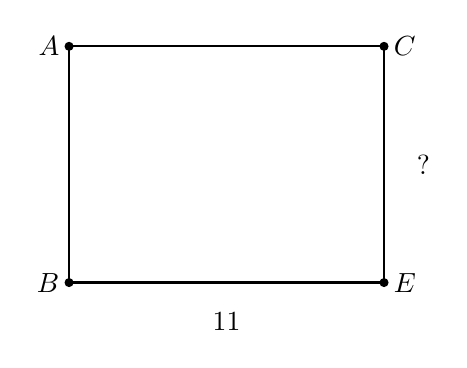
\begin{tikzpicture}
    \draw [-, thick] (0,0)--(4,0)--(4,3)--(0,3)--cycle;
    \draw [fill] (0,0) circle [radius=0.05] node[left]{$B$};
    \draw [fill] (4,0) circle [radius=0.05] node[right]{$E$};
    \draw [fill] (4,3) circle [radius=0.05] node[right]{$C$};
    \draw [fill] (0,3) circle [radius=0.05] node[left]{$A$};
    \node at (4.5, 1.5){?};
    \node at (2, -0.5){11};
  \end{tikzpicture}
  \end{flushright}


\item Find the area and perimeter of the shape shown below. Mark the missing side lengths first. All angles are $90^\circ$.\hfill \emph{(not drawn to scale)}
\begin{flushleft}
\begin{tikzpicture}[rotate=90]
  \draw [-, thick] (0,0)--(5,0)--(5,2)--(3,2)--(3,6)--(0,6)--cycle;
  %\draw [fill] (0,0) circle [radius=0.05] node[left]{$A$};
  %\draw [fill] (7,0) circle [radius=0.05] node[right]{$B$};
  %\draw [fill] (7,2) circle [radius=0.05] node[right]{$C$};
  %\draw [fill] (0,2) circle [radius=0.05] node[left]{$D$};
  \node at (5.5, 1){3};
  \node at (4, 2.5){4};
  \node at (2.5, -0.5){10};
  \node at (-0.5, 3){13};
\end{tikzpicture}
\end{flushleft} \vspace{1cm}

\item Find the area $A$ and circumference $C$ of a circle with radius 4 meters (in terms of $\pi$). 
  
\newpage
\item Find the area of $\triangle ABC$. The altitude $h$ of the triangle is $8$ centimeters and the base $AB=10 \frac{1}{2}$ cm. (diagram not to scale) \\[0.5cm]
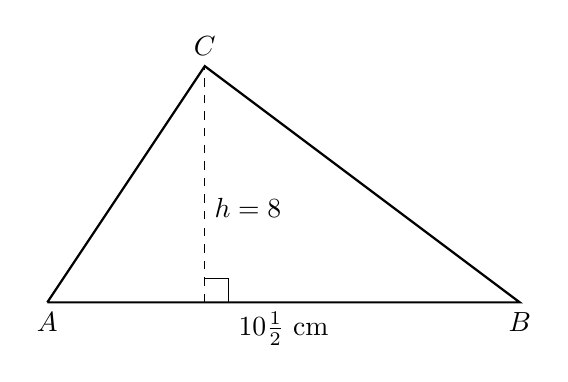
\begin{tikzpicture}[scale=1.]
  \draw [thick]
    (2,0)node[below]{$A$}--
    (8,0)node[below]{$B$}--
    (4,3)node[above]{$C$} --(2,0);
 \draw [dashed] (4,0)--(4,3);
 \draw (4,0)++(0.3,0)--++(0,0.3)--+(-0.3,0);
 \node at (4,1.2)[right]{$h=8$};
 \node at (5,0)[below]{$10 \frac{1}{2}$ cm};
\end{tikzpicture} 

\item The compound shape shown below is composed of a rectangle 3 inches by 7 inches, and a triangle with base 2 inches. Find the total area of the combined shape.
    \vspace{0.5cm} 
    \begin{flushleft}
    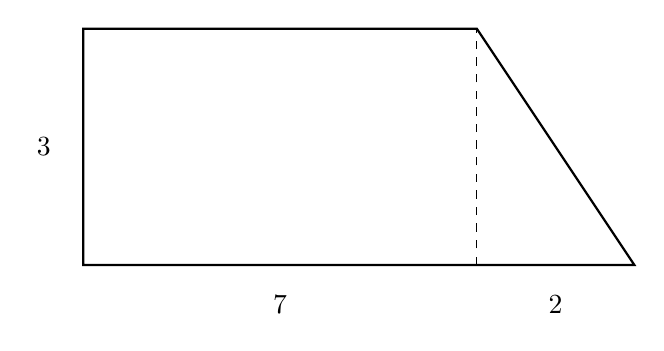
\begin{tikzpicture}
      \draw [-, thick] (0,0)--(7,0)--(5,3)--(0,3)--cycle;
      \draw [dashed] (5,0)--(5,3);
      %\draw [fill] (0,0) circle [radius=0.05] node[left]{$A$};
      %\draw [fill] (7,0) circle [radius=0.05] node[right]{$B$};
      %\draw [fill] (7,2) circle [radius=0.05] node[right]{$C$};
      %\draw [fill] (0,2) circle [radius=0.05] node[left]{$D$};
      \node at (6, -0.5){2};
      \node at (2.5, -0.5){7};
      \node at (-0.5, 1.5){3};
    \end{tikzpicture}
    \end{flushleft}
        
  \item The area of a square is 36 square centimeters. Find the length of the side of the square. \vspace{3cm}


  \item One side of the $\triangle ABC$ has a length $AB=12$. The triangle's area is 60. Find the length of the altitude $h$ of the triangle to vertex $C$ and perpendicular to side $\overline{AB}$.\\
  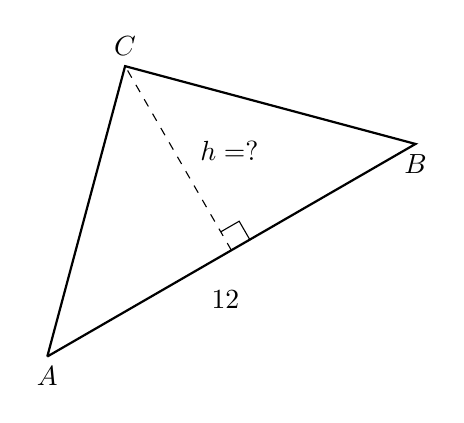
\begin{tikzpicture}[scale=0.9, rotate=30]
    \draw [thick]
      (2,0)node[below]{$A$}--
      (8,0)node[below]{$B$}--
      (5,3)node[above]{$C$} --(2,0);
    \draw [dashed] (5,0)--(5,3);
    \draw (5,0)++(0.3,0)--++(0,0.3)--+(-0.3,0);
    \node at (5.2,1.5)[right]{$h=?$};
    \node at (5,-0.5)[below left]{$12$};
  \end{tikzpicture}
  
\end{enumerate}
\end{document}